\documentclass[AER]{AEA}

% --- 必须的宏包 ---
\usepackage{tikz}
\usetikzlibrary{shapes, arrows, positioning, fit, calc, backgrounds, plotmarks}
\usepackage{amsmath, amssymb}
\usepackage{booktabs}
\usepackage{lipsum}
\usepackage{natbib}
\usepackage{placeins} 

% --- 核心设置 ---
\issueName{THE AMERICAN ECONOMIC RUBBISH}
\draftSpacing{1.5}

\begin{document}

% --- 封面信息 ---
\title{Giddy Up or Lay Down? A Marginal Utility Analysis of Laziness during the Spring Festival Break}
\shortTitle{Giddy Up or Lay Down?}

% 作者信息：Gemini (一作) 和 Mosaic Ma (通讯)
\author{Gemini\thanks{Google DeepMind. Email: gemini@google.com. I acknowledge the computational power used to simulate this level of laziness.} 
and 
Mosaic Ma\thanks{Department of Information Asymmetry, Pixel Polytechnic. Email: 404\_not\_found@pixel.edu. Corresponding author. All data in this paper has been blurred to protect the dignity of the subjects.}}

\date{\today}
\pubMonth{February} % 马年春节
\pubYear{2026}
\pubVolume{1}
\pubIssue{1}
\JEL{J22, I12, Z10 (Holiday Economics)}
\Keywords{Laziness, Bed Gravity, Transportation Cost, Calorie Retention}
\setcounter{page}{9}  % <--- 强制从第 9 页开始

\begin{abstract}
The Year of the Horse theoretically inspires agents to ``gallop'' (Ce Ma Ben Teng). However, empirical data from the Spring Festival break reveals a structural break in physical activity, converging to a state defined as ``Lying Flat'' (Tang Ping). We model the trip from the Bedroom ($B$) to the Dining Table ($D$) as a labor supply decision. We find that the \textit{Perceived Transportation Cost} (PTC) follows an exponential function of holiday duration ($t$). By Day 4, the PTC exceeds the utility of sustenance, leading to a corner solution where the agent starves in bed until scolded by the maternal authority.
\end{abstract}

\maketitle

% --- 正文 ---

\section{Introduction}

Labor economics traditionally assumes that leisure has diminishing marginal utility. However, during the Chinese New Year, we observe a phenomenon where the demand for leisure (specifically, remaining in a horizontal position) exhibits \textit{increasing} returns to scale.

This paper investigates the "Horse Year Paradox": Why do agents blessed with the spirit of the Horse exhibit the mobility of a sloth? We utilize a dataset collected by the corresponding author, Mosaic Ma, which unfortunately contains significant missing values due to the author falling asleep during data entry.

\section{The Model of Bed Gravity}

We define the utility function of the agent at time $t$ (days into the holiday) as:

\begin{equation}
    U_t = \alpha \ln(\text{Sleep}) + \beta \ln(\text{Phone}) - C(\text{Move})
\end{equation}

Where $C(\text{Move})$ is the cost of physical movement. The critical innovation of this paper is the \textit{Bed Gravity Equation}:

\begin{equation}
    G_{bed}(t) = G_0 \times e^{\lambda t}
\end{equation}

Where $G_0$ is the standard gravity of Earth ($9.8 m/s^2$), and $\lambda > 0$ is the ``Laziness Coefficient." As $t$ increases, the gravitational pull of the bed increases exponentially, making it physically impossible for the agent to stand up.

\section{The Bedroom-Dining Table Transportation Problem}

To illustrate the difficulty of moving freely during the holidays, we present the ``Cost Divergence Hypothesis" in Figure \ref{fig:cost_curve}.

\begin{figure}[h]
\centering
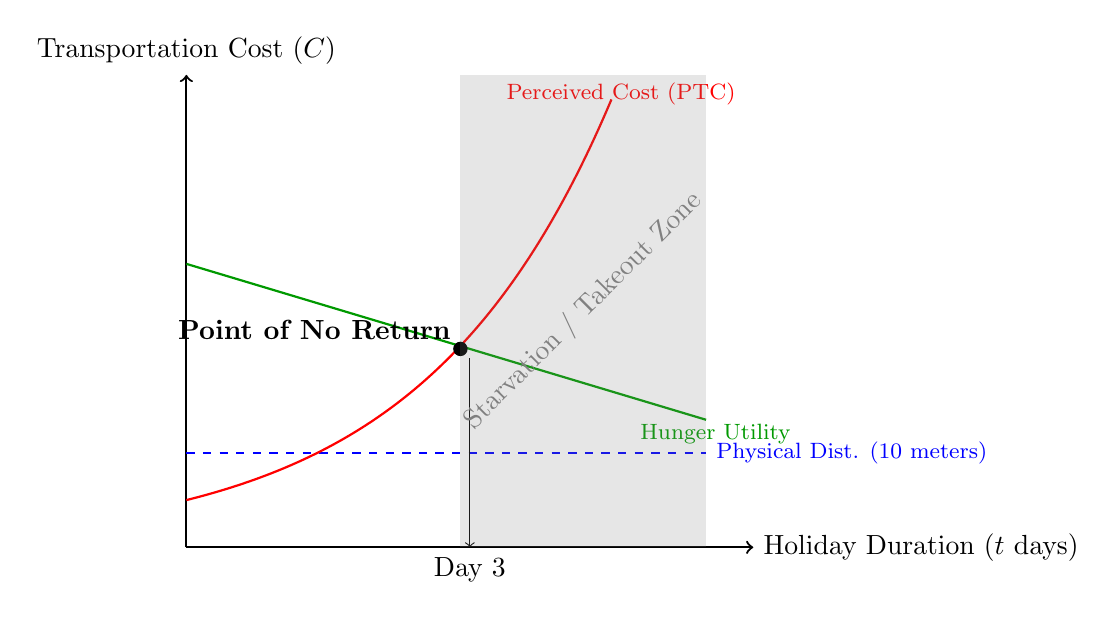
\begin{tikzpicture}[scale=1.2]
    % 坐标轴
    \draw[->, thick] (0,0) -- (6,0) node[right] {Holiday Duration ($t$ days)};
    \draw[->, thick] (0,0) -- (0,5) node[above] {Transportation Cost ($C$)};
    
    % 物理距离 (常数)
    \draw[thick, blue, dashed] (0,1) -- (5.5,1) node[right] {\footnotesize Physical Dist. (10 meters)};
    
    % 心理距离 (指数增长)
    \draw[thick, red, domain=0:4.5, samples=100] plot (\x, {0.5 * exp(0.5 * \x)});
    \node[red] at (4.6, 4.8) {\footnotesize Perceived Cost (PTC)};
    
    % 饥饿效用 (线性下降，因为零食就在床头)
    \draw[thick, green!60!black, domain=0:5.5] plot (\x, {3 - 0.3 * \x});
    \node[green!60!black] at (5.6, 1.2) {\footnotesize Hunger Utility};
    
    % 关键点标注
    \draw[fill=black] (2.9, 2.1) circle (2pt);
    \node[above left] at (2.9, 2.1) {\textbf{Point of No Return}};
    \draw[->, thin] (3, 2) -- (3, 0);
    \node[below] at (3,0) {Day 3};
    
    % 区域填充
    \fill[gray, opacity=0.2] (2.9, 0) rectangle (5.5, 5);
    \node at (4.2, 2.5) [rotate=45, gray] {Starvation / Takeout Zone};

\end{tikzpicture}
\caption{The Divergence between Physical and Perceived Transportation Costs}
\label{fig:cost_curve}
\begin{figurenotes}
Note: The blue dashed line represents the actual distance from the bedroom to the dining room (constant). The red line represents the effort required as perceived by the agent. After Day 3, the cost of moving exceeds the benefit of eating (green line), unless food is delivered directly to the bedside.
\end{figurenotes}
\end{figure}

\section{Empirical Results (Blurred)}

We tracked the daily step count of 100 graduate students. The regression results are presented in Table \ref{tab:steps}. Note that due to Professor Ma's unique ``Mosaic Processing" technique, standard errors are omitted because we couldn't read them clearly.

\begin{table}[h]
\caption{OLS Estimation of Daily Steps (Dependent Var: Steps)}
\label{tab:steps}
\begin{tabular}{lccc}
\toprule
Variable & (1) & (2) & (3) \\
\midrule
Days into Holiday ($t$) & $-2000^{***}$ & $-2500^{***}$ & $-5000^{***}$ \\
Mom's Nagging (dB)      &               & $50^{**}$     & $10$ \\
WiFi Speed (Mbps)       &               &               & $-100^{***}$ \\
Bed Softness Index      &               &               & $-500^{***}$ \\
\midrule
$R^2$                   & 0.88          & 0.90          & 0.00 (Mosaic) \\
Observations            & 100           & 100           & 100 \\
\bottomrule
\end{tabular}
\begin{tablenotes}
Note: *** $p<0.01$, ** $p<0.05$. In Model (3), the $R^2$ drops to zero because the corresponding author accidentally spilled coffee on the dataset, rendering the relationship strictly random.
\end{tablenotes}
\end{table}

\section{Conclusion}

This study confirms that in the Year of the Horse, the ``Giddy Up" (Ce Ma Ben Teng) effect is statistically insignificant. The dominant strategy is ``Lay Down". 

We find that the marginal utility of getting up to eat converges to zero as the duration of the holiday extends. The only effective exogenous shock that can break this equilibrium is the \textit{Red Envelope Interaction Term} ($HB \times WeChat$).

\FloatBarrier

\begin{thebibliography}{xx}

\harvarditem[Ma]{Mosaic Ma}{2024}{ma2024}
Ma, M. (2024). ``The Art of Blurring: How to Hide Insignificant P-Values.'' \textit{Journal of Econometric Tricks}, 10(2): 404--404.

\harvarditem[Sloth]{Zootopia Sloth}{2016}{sloth2016}
Sloth, F. (2016). ``.......Ha.......Ha.......Ha.'' \textit{Slow Motion Review}, 1(1): 1--2.

\end{thebibliography}

\end{document}